\documentclass{article}
\usepackage{cmap}
\usepackage[utf8]{inputenc}
\usepackage{graphicx}
\usepackage[colorlinks=true]{hyperref}

\title{Report}
\author{Thorvald Demuth Jørgensen}
\date{\today} 

\begin{document}
\maketitle 


\section{Første afsnit} 
Vi startede ud med at lave følgende program \\

\begin{figure}[h]
	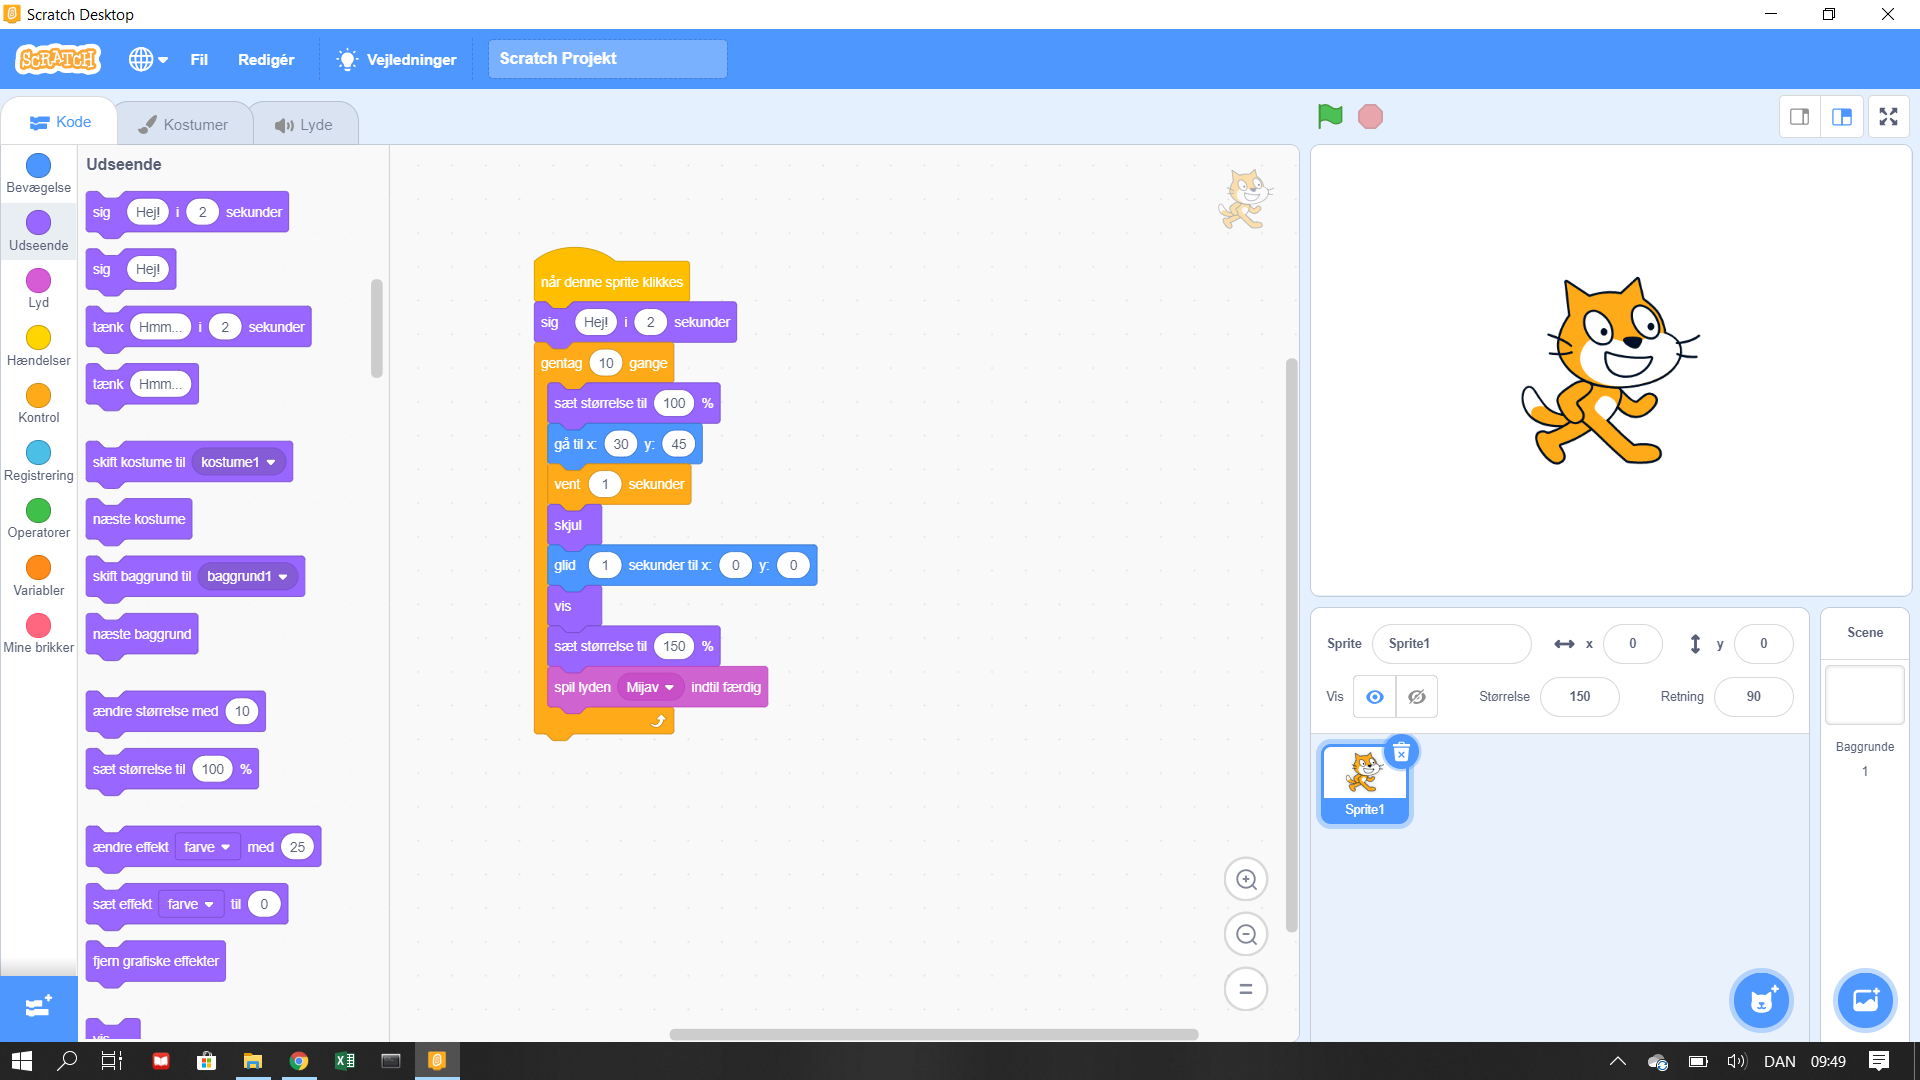
\includegraphics[width=\linewidth]{1billede.png}
\end{figure}

Vi havde en forventning om at når vi klikkede på katten, ville den sige hej og derfra gentagende gange glide til punktet (30,45) vente et øjeblik, poppe op et nyt sted større og sige Miav. \\
Da vi endte med at køre programet fandt vi ud af at katten ikke gled hen af skærmen, men blot poppede op det ene sted og poppede op et andet. \\
Vi redigerede så programet til følgende: \\

\begin{figure}[h]
	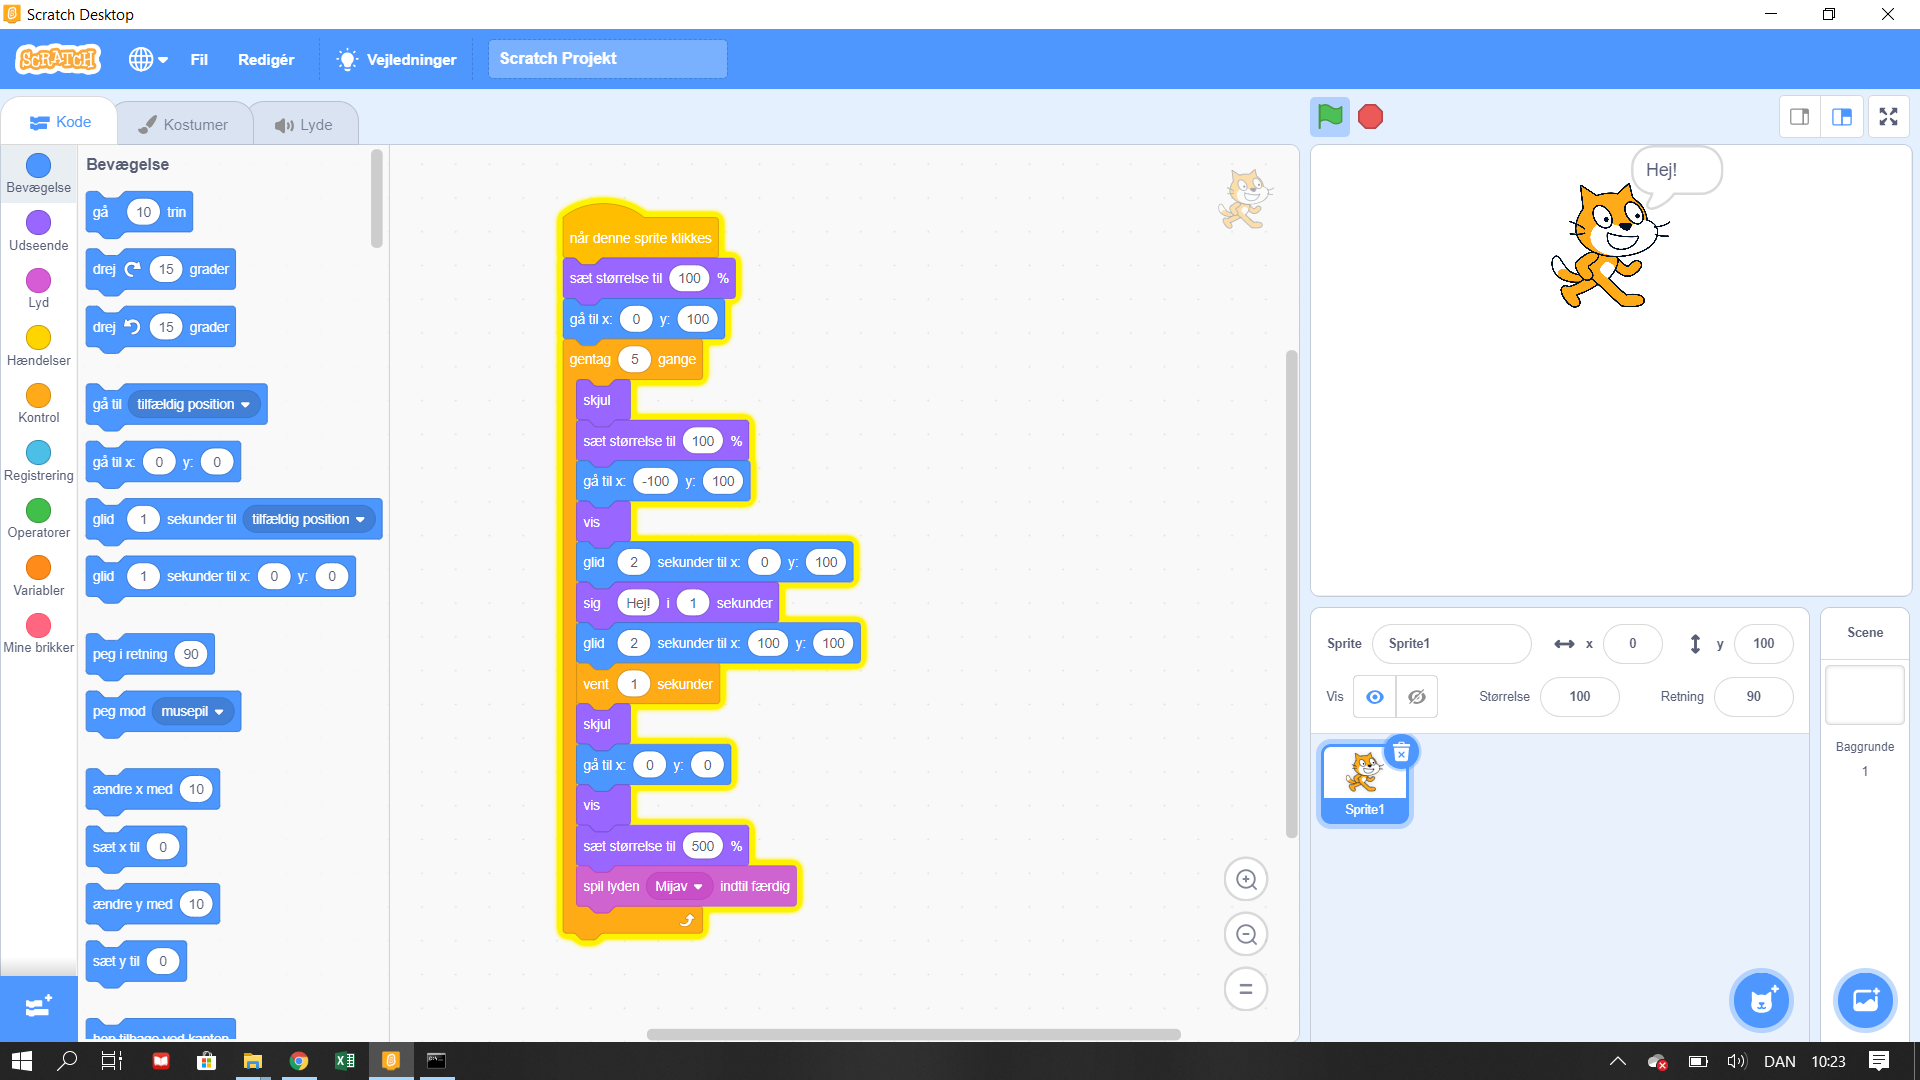
\includegraphics[width=\linewidth]{2billede.png}
\end{figure}

Hvor der nu kom en meget bedre bevægelse af en kat, der går en tur og popper op på skærmen tæt på brugeren og siger "Miav"..

\section{Spil}
\begin{figure}[h]
	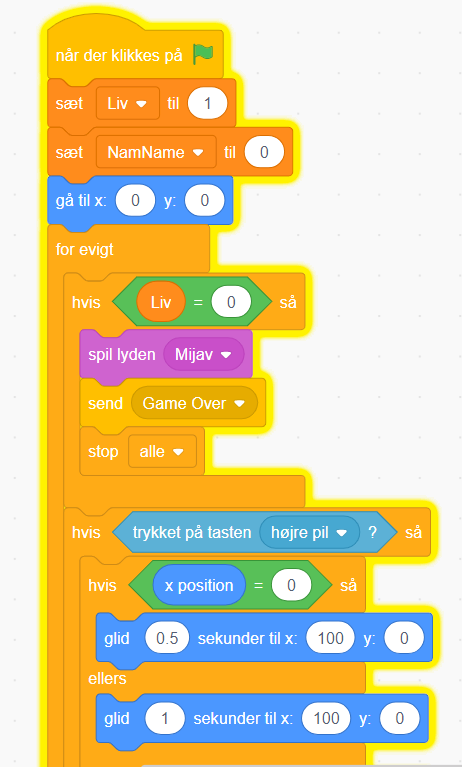
\includegraphics[scale=0.2]{3billede.png}
\end{figure}

\begin{figure}[h]
	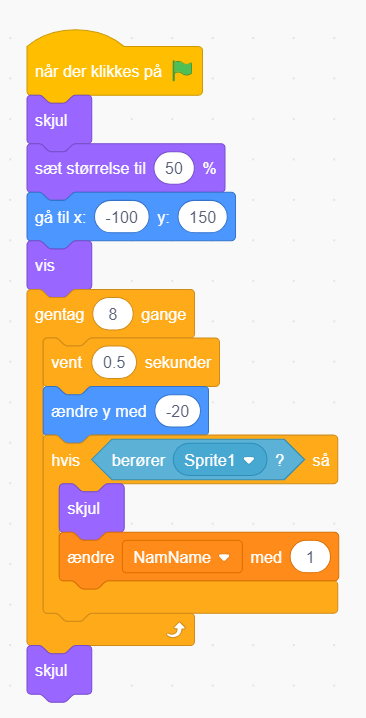
\includegraphics[scale=0.2]{4billede.png}
\end{figure}

\end{document}
